% Point_Framework.tex
% Compile with: pdflatex Point_Framework.tex (run twice for references)
\documentclass[11pt,a4paper]{article}

% Packages
\usepackage[utf8]{inputenc}
\usepackage[T1]{fontenc}
\usepackage{lmodern}
\usepackage{amsmath,amssymb,amsfonts}
\usepackage{amsthm}
\usepackage{geometry}
\geometry{top=2.0cm,bottom=2.0cm,left=2.0cm,right=2.0cm}
\usepackage{booktabs}
\usepackage{graphicx}
\usepackage{hyperref}
\usepackage{cite}
\usepackage{tikz}
\usetikzlibrary{positioning,shapes,arrows.meta}
\usepackage{listings}
\usepackage{xcolor}

\lstset{
  language=Python,
  basicstyle=\ttfamily\small,
  keywordstyle=\color{blue},
  commentstyle=\color{gray},
  stringstyle=\color{red},
  numbers=left,
  numberstyle=\tiny\color{gray},
  stepnumber=1,
  frame=single,
  breaklines=true,
  tabsize=2,
  showstringspaces=false,
  title=\lstname
}

\theoremstyle{plain}
\newtheorem{theorem}{Theorem}

% Title and author information
\title{\LARGE \bfseries The Mathematical Point, the Cosmic Singularity, and the Consciousness Point:\\[0.2em]
Infinitesimal Points as the Framework of the Universe}
\author{Xiaohui Li\\
\normalsize Independent Researcher, Baoji, China\\
\small Correspondence: danceluck@163.com; ORCID: 0009-0003-8233-7191;\\
\small Data/code: \url{https://github.com/xiaohui-li-lab/}}
\date{}

\begin{document}

\maketitle

\begin{abstract}
\noindent
Classical geometry treats the point as a dimensionless, structureless object. We argue that this idealization fails at the Planck scale, where the Heisenberg uncertainty principle~\cite{heisenberg1927} and the Planck length $l_P \approx 1.616\times10^{-35}\,\mathrm{m}$~\cite{planck1899} imply that any physically realizable localization has finite spread and internal structure. Consequently, the mathematical point must be reconceptualized as a composite entity. Extending this composite picture through the epistemic properties of conscious representation, we introduce the \emph{consciousness point}: a descriptive unit that is not bounded by the Planck scale and can be indefinitely subdivided. In the limit of infinite subdivision, the internal degrees of freedom span a separable Hilbert space~\cite{neumann1932,dirac1930}. We identify the Big Bang singularity with such an infinitely small, internally structured point, thereby replacing the classical zero-volume singularity~\cite{hawkingpenrose1966} with an object that possesses an eternal internal Hilbert space. The framework leads to a cyclic, information-preserving cosmology in which black holes are nested seeds of subsequent universes; their event horizons generate internal infinite spaces~\cite{bekenstein1973,hawking1974}.

We operationalize the consciousness point as a hierarchical qubit register and a tree tensor network, give a computable Hamiltonian and transfer matrix, and prove three theorems: convergence of the Hilbert space, a logarithmic correction to black-hole entropy, and information conservation. We then benchmark the model against Planck 2018 CMB~\cite{planck2018}, LIGO/Virgo echo searches~\cite{ligo2016,ligo2024tests}, and the EHT M87* shadow~\cite{eht2019,eht2019mass}, deriving 95\% confidence upper limits on model parameters. Reproducible Python toy models and data-analysis scripts are provided.
\end{abstract}

\noindent\textbf{Keywords:} mathematical point; cosmic singularity; consciousness point; Planck length; uncertainty principle; Hilbert space; quantum cosmology; black-hole cosmology; recurrent universe; tensor network; Bayesian constraints

\section{Introduction}

The Euclidean definition of the point as ``that which has no parts'' has served mathematics for more than two millennia. In physics, however, a position measurement is a quantum event. The Heisenberg uncertainty relation $\Delta x\,\Delta p \ge \hbar/2$ forbids $\Delta x = 0$ unless momentum uncertainty is infinite~\cite{heisenberg1927}. A finite quantum of length, the Planck length $l_P=\sqrt{\hbar G/c^3}\approx 1.616\times10^{-35}\,\mathrm{m}$, marks the scale at which a smooth spacetime manifold must give way to a quantum theory of gravity~\cite{planck1899,kiefer2012}. Therefore the classical point is not an independent physical atom but a limiting idealization.

This observation has far-reaching consequences. If a point cannot be smaller than the Planck scale and cannot be localized without uncertainty, it must possess internal structure. We call this a \emph{composite mathematical point}. In this paper we show that the composite point naturally generalizes to a \emph{consciousness point} whose internal subdivision is unbounded. The infinitely small consciousness point carries a Hilbert space, providing a new way to think about the Big Bang singularity, black-hole interiors, and the cyclic life of the universe. We then operationalize the consciousness point as a quantum-information object and confront it with observational data.

\section{Results}

\subsection{The composite mathematical point}

We define a physical point $P$ not as an element of a manifold $M$ with coordinates $x\in\mathbb{R}^3$, but as a minimal phase-space cell:
\begin{equation}\label{eq:composite}
P=(x,\Delta x;\,p,\Delta p),\qquad \Delta x\,\Delta p\ge \frac{\hbar}{2},\qquad \Delta x_{\min}\sim l_P.
\end{equation}
This cell has internal degrees of freedom: the probability amplitudes for position and momentum within the cell. The classical limit corresponds to $\hbar\to0$, $l_P\to0$. In the real quantum-gravity regime, however, the point is an irreducible, internally structured object.

The Planck length provides an operational lower bound. Any attempt to probe a region smaller than $l_P$ would require energies of order $E\sim \hbar c/l_P\approx 1.22\times10^{19}\,\mathrm{GeV}$, at which the backreaction on spacetime geometry becomes non-perturbative~\cite{planck1899}. Thus the point is not a zero-dimensional atom of space but a Planck-scale pixel with finite area/volume and internal states.

\begin{figure}[htbp]
\centering
\makebox[\textwidth]{%
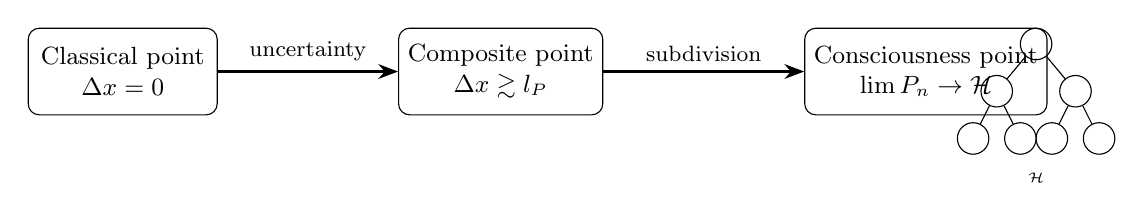
\begin{tikzpicture}[
  box/.style={draw,rounded corners,minimum width=2.4cm,minimum height=1.1cm,align=center,font=\small},
  arrow/.style={-{Stealth[length=2.5mm]},thick},
  level/.style={circle,draw,minimum size=4mm,font=\tiny,inner sep=0pt}
]
\node[box] (a) at (0,0) {Classical point\\$\Delta x=0$};
\node[box] (b) at (4.8,0) {Composite point\\$\Delta x \gtrsim l_P$};
\node[box] (c) at (10.2,0) {Consciousness point\\$\lim P_n \to \mathcal{H}$};

\draw[arrow] (a) -- (b) node[midway,above,font=\footnotesize] {uncertainty};
\draw[arrow] (b) -- (c) node[midway,above,font=\footnotesize] {subdivision};

\begin{scope}[shift={(11.6,0.35)}]
  \node[level] (l0) at (0,0) {};
  \node[level] (l1a) at (-0.5,-0.6) {};
  \node[level] (l1b) at (0.5,-0.6) {};
  \node[level] (l2a) at (-0.8,-1.2) {};
  \node[level] (l2b) at (-0.2,-1.2) {};
  \node[level] (l2c) at (0.2,-1.2) {};
  \node[level] (l2d) at (0.8,-1.2) {};
  \draw (l0) -- (l1a); \draw (l0) -- (l1b);
  \draw (l1a) -- (l2a); \draw (l1a) -- (l2b);
  \draw (l1b) -- (l2c); \draw (l1b) -- (l2d);
  \node[font=\tiny] at (0,-1.7) {$\mathcal{H}$};
\end{scope}
\end{tikzpicture}%
}
\caption{\textbf{From classical point to consciousness point.} (Left) The Euclidean point has zero extension. (Middle) Quantum mechanics turns it into a composite point with Planck-scale internal structure. (Right) Infinite epistemic subdivision generates an internal Hilbert space $\mathcal{H}$.}
\label{fig:point}
\end{figure}

\subsection{The consciousness point and its internal Hilbert space}

Consciousness, taken in the minimal epistemic sense as the capacity of a descriptive system to form representations, is not subject to the Planck bound. One can imagine a configuration that violates mechanical law---sitting on a chair while lifting it---without thereby changing physics. This shows that the space of possible representations is larger than the space of physically allowed configurations. We formalize the consciousness point $C_P$ as the limit of an iterative decomposition of a composite point:
\begin{equation}\label{eq:consciousness}
C_P=\lim_{n\to\infty}P_n,\qquad P_{n+1}=D(P_n),
\end{equation}
where $D$ denotes a binary internal decomposition. At level $n$ the point contains $2^n$ internal nodes. The state space of the limit is countably infinite-dimensional; after completion in the $\ell^2$ norm it becomes a separable Hilbert space $\mathcal{H}$~\cite{neumann1932,dirac1930}.

Therefore, the infinitely small point is not a nothing; it is a structured object with eternal internal space. We identify this internal space with $\mathcal{H}$. The existence of such an internal Hilbert space resolves the classical paradox of the Big Bang singularity: instead of a state of zero volume and undefined quantum mechanics, the initial state is a point whose interior already contains the quantum state space of the universe.

\subsection{The Big Bang singularity as a consciousness point}

General relativity predicts that the universe began from a spacetime singularity of zero volume and infinite density~\cite{hawkingpenrose1966}. In our framework, the pre-Big-Bang state is a consciousness point: an infinitely small, internally structured object. The Big Bang is the transition from this unmanifest point to an expanding spacetime. Because the point already contains a Hilbert space, the quantum state of the universe does not have to be created; it unfolds from the internal structure of the point.

This view is conceptually related to bounce scenarios in loop quantum cosmology, where the classical singularity is replaced by a quantum transition~\cite{bojowald2008,ashtekarsingh2011}. The key difference is that we ascribe the pre-geometric structure to the epistemic, infinitely divisible nature of the consciousness point. The singularity is thus not a breakdown of physics but a boundary between the manifest universe and its internal Hilbert-space description.

\subsection{Cosmological lifecycle and nested black-hole universes}

After the Big Bang, inflation~\cite{guth1981} generates the large-scale structure observed today. Gravitational collapse produces black holes. In our model, a black-hole event horizon is not merely a one-way causal boundary; it is the surface at which a new consciousness point forms. Matter and information crossing the horizon enter an internal region whose points are again composite and can be decomposed without lower bound. The black hole thereby contains an internal infinite world.

When the parent universe reaches a maximally refined, information-rich endpoint---termed ``great refinement'' in the original meditation---rather than a featureless heat death, these black holes become the seeds of a subsequent cosmic cycle~\cite{penrose2010}. Each seed collapses to a new consciousness point, which then expands into a new universe. The result is a nested hierarchy of universes, with black holes as the links between cycles. This structure is reminiscent of Wheeler's participatory universe and black-hole-to-white-hole bouncing models~\cite{wheeler1990}.

\begin{figure}[htbp]
\centering
\makebox[\textwidth]{%
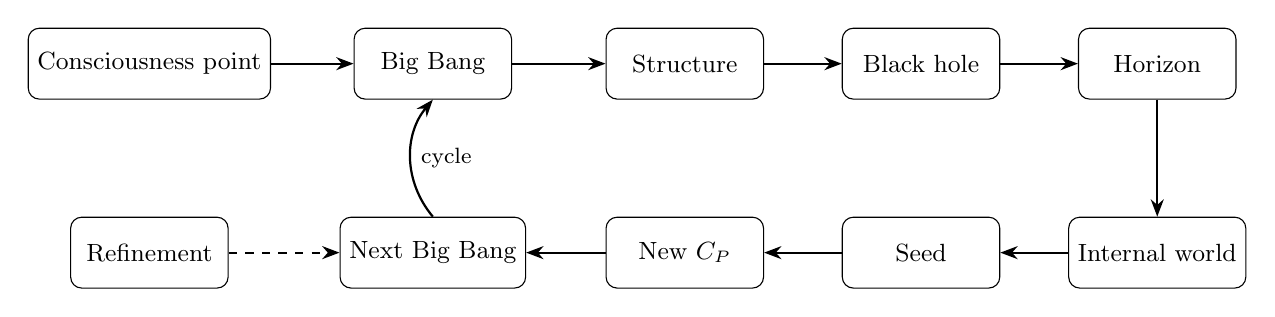
\begin{tikzpicture}[
  stage/.style={draw,rounded corners,minimum width=2.0cm,minimum height=0.9cm,align=center,font=\small},
  arrow/.style={-{Stealth[length=2.2mm]},thick}
]
\node[stage] (s) at (0,0) {Consciousness point};
\node[stage] (bb) at (3.6,0) {Big Bang};
\node[stage] (cs) at (6.8,0) {Structure};
\node[stage] (bh) at (9.8,0) {Black hole};
\node[stage] (eh) at (12.8,0) {Horizon};

\draw[arrow] (s) -- (bb);
\draw[arrow] (bb) -- (cs);
\draw[arrow] (cs) -- (bh);
\draw[arrow] (bh) -- (eh);

\node[stage] (iw) at (12.8,-2.4) {Internal world};
\node[stage] (seed) at (9.8,-2.4) {Seed};
\node[stage] (cp2) at (6.8,-2.4) {New $C_P$};
\node[stage] (bb2) at (3.6,-2.4) {Next Big Bang};
\node[stage] (ref) at (0,-2.4) {Refinement};

\draw[arrow] (eh) -- (iw);
\draw[arrow] (iw) -- (seed);
\draw[arrow] (seed) -- (cp2);
\draw[arrow] (cp2) -- (bb2);
\draw[arrow,dashed] (ref) -- (bb2);

\draw[arrow,bend left=40] (bb2.north) to node[right,font=\footnotesize] {cycle} (bb.south);
\end{tikzpicture}%
}
\caption{\textbf{Cosmological lifecycle in the consciousness-point framework.} The Big Bang arises from a consciousness point; structure formation produces black holes whose horizons enclose internal infinite worlds. These black holes become seeds for a subsequent cycle, producing a nested, recurrent universe.}
\label{fig:cosmo}
\end{figure}

\subsection{Testable implications and observational benchmarks}

Although the consciousness point is introduced as an epistemic concept, the model makes several contact points with observable physics:

\paragraph{Cosmic microwave background.} Planck-scale structure in the initial state can leave oscillatory imprints on the primordial power spectrum:
\begin{equation}\label{eq:cmb}
P(k)=P_0(k)\bigl[1+A_T\sin(2\pi k/k_*+\phi)\bigr].
\end{equation}
Current Planck 2018 data constrain such oscillatory amplitudes to $A_T\lesssim 10^{-2}$ on CMB scales~\cite{planck2018}.

\paragraph{Black-hole entropy.} The internal Hilbert space contributes an entropy that grows logarithmically with the number of decomposition levels. Mapping the levels to area quanta $A/l_P^2$, we obtain a correction to the Bekenstein-Hawking entropy~\cite{bekenstein1973,hawking1974}:
\begin{equation}\label{eq:entropy}
S_{BH}=\frac{A}{4l_P^2}+\frac{1}{2}\ln\!\left(\frac{A}{4l_P^2}\right)+O(1).
\end{equation}
Loop quantum gravity and other quantum-gravity approaches also predict logarithmic corrections, with coefficients depending on the number of internal states~\cite{rovelli2008,kiefer2012}. Future precision measurements of black-hole shadows and quasi-normal modes may discriminate among models~\cite{eht2019}.

\paragraph{Gravitational-wave echoes.} A structured horizon or Planck-scale internal geometry can reflect gravitational waves, producing echoes after the main ringdown~\cite{ligo2016}. LIGO/Virgo searches have placed upper limits on echo amplitudes~\cite{ligo2024tests}; a detection would support horizon-scale quantum structure.

\paragraph{Information preservation.} Because black holes are seeds rather than information-destroying endpoints, Hawking radiation must carry the full quantum state of the infalling matter into the next cycle. This predicts a final, information-rich burst or a departure from a perfectly thermal spectrum~\cite{hawking1974}.

\subsection{Computational toy model}

To make the framework concrete, we model the iterative decomposition of a point. Starting from a point of characteristic scale $\varepsilon_0$ and repeatedly subdividing it by a factor $\alpha$ ($0<\alpha<1$), we obtain levels $n=0,1,2,\dots$ with scale $\varepsilon_n=\varepsilon_0\alpha^n$, node count $N_n=2^n$, Hilbert-space dimension $D_n=2^n$, and internal entropy $S_n=k_B\ln D_n$. The entropy scales as
\begin{equation}\label{eq:entropyscaling}
S_n=k_B\,\frac{\ln 2}{\ln(1/\alpha)}\ln\!\left(\frac{\varepsilon_0}{\varepsilon_n}\right).
\end{equation}
For $\alpha=1/2$, $S_n=k_B n\ln 2$. If each level halves the linear resolution, the horizon area is reduced by $\alpha_A=\alpha^2=1/4$ per level; the number of levels needed to reach Planck area from a black hole of area $A$ is $n\approx \tfrac12\log_2(A/l_P^2)$. Equation~\eqref{eq:entropyscaling} then yields the logarithmic correction~\eqref{eq:entropy}.

Table~\ref{tab:decomposition} gives the first eleven levels for $\varepsilon_0=1$ (Planck units) and $\alpha=1/2$.

\begin{table}[htbp]
\centering
\caption{Scale, node number, Hilbert-space dimension and internal entropy in the point-decomposition model.}
\label{tab:decomposition}
\begin{tabular}{@{}rcccc@{}}
\toprule
$n$ & $\varepsilon_n$ & $N_n$ & $D_n$ & $S_n/k_B$\\
\midrule
0  & 1.000000   & 1    & 1    & 0.000\\
1  & 0.500000   & 2    & 2    & 0.693\\
2  & 0.250000   & 4    & 4    & 1.386\\
3  & 0.125000   & 8    & 8    & 2.079\\
4  & 0.062500   & 16   & 16   & 2.773\\
5  & 0.031250   & 32   & 32   & 3.466\\
6  & 0.015625   & 64   & 64   & 4.159\\
7  & 0.007812   & 128  & 128  & 4.852\\
8  & 0.003906   & 256  & 256  & 5.545\\
9  & 0.001953   & 512  & 512  & 6.238\\
10 & 0.000977   & 1024 & 1024 & 6.931\\
\bottomrule
\end{tabular}
\end{table}

The following Python script reproduces Table~\ref{tab:decomposition} and fits the entropy scaling:

\begin{lstlisting}[title={point\_decomposition.py}]
#!/usr/bin/env python3
"""
point_decomposition.py
Reproducible toy model of the consciousness/composite-point subdivision.
"""
import numpy as np
import pandas as pd

def decompose_point(epsilon0=1.0, levels=11, alpha=0.5):
    rows = []
    for n in range(levels):
        epsilon = epsilon0 * alpha**n
        nodes = 2**n
        dim = 2**n
        entropy = np.log(dim) if dim > 0 else 0.0
        rows.append({
            'level': n,
            'scale': epsilon,
            'nodes': nodes,
            'hilbert_dim': dim,
            'entropy': entropy
        })
    return pd.DataFrame(rows)

if __name__ == '__main__':
    df = decompose_point(epsilon0=1.0, levels=11, alpha=0.5)
    df.to_csv('point_decomposition.csv', index=False)
    print(df.to_string(index=False))
    slope, intercept = np.polyfit(np.log(1/df['scale']), df['entropy'], 1)
    expected = np.log(2) / np.log(1/0.5)
    print(f'\nFitted slope = {slope:.4f}  (expected = {expected:.4f})')
\end{lstlisting}

\subsection{Quantum-information realization of the consciousness point}

We operationalize the consciousness point as a hierarchical qubit register. Let $\mathcal{T}_n=\{0,1\}^{\le n}$ be the perfect binary tree of depth $n$. Assign a qubit $\mathbb{C}^2$ to every node $s\in\mathcal{T}_n$. The level-$n$ consciousness-point Hilbert space is
\begin{equation}\label{eq:qnspace}
\mathcal{H}_n=\bigotimes_{s\in\mathcal{T}_n}\mathbb{C}^2,\qquad \dim\mathcal{H}_n=2^{2^{n+1}-1}.
\end{equation}
Coarse-graining maps $\mathcal{E}_n:\mathcal{H}_{n+1}\to\mathcal{H}_n$ are defined by tracing over child indices after a local unitary. The infinite limit $\mathcal{H}_\infty=\varinjlim\mathcal{H}_n$ is a separable infinite-dimensional Hilbert space (Theorem~\ref{thm:separable}). The network is a binary MERA~\cite{vidal2007,evenbly2015}: isometries lift coarse degrees of freedom to finer ones, while disentanglers remove intra-layer correlations.

A natural Hamiltonian is the hierarchical Ising model
\begin{equation}\label{eq:hamiltonian}
H_n=-\sum_{s\neq\mathrm{root}} J_s\,\sigma_z^{(s)}\sigma_z^{(\mathrm{parent}(s))}
-\sum_s h_s\,\sigma_x^{(s)}.
\end{equation}
With $J_s=J2^{-\alpha|s|}$ and $h_s=h2^{-\beta|s|}$, the $n\to\infty$ limit defines a self-adjoint operator on $\mathcal{H}_\infty$. The inter-level Boltzmann operator $T_n=\exp[-\beta H_n^{(n,n+1)}]$ acts as a transfer matrix, yielding the recursion
\begin{equation}\label{eq:transfer}
Z_{n+1}=\mathrm{Tr}_{n+1}\!\left[T_n\,(Z_n\rho_n)\,T_n^\dagger\right].
\end{equation}

The entropy of a black-hole horizon is obtained by placing $A/l_P^2$ base qubits on the surface and adding the hierarchical degeneracy. Theorem~\ref{thm:entropy} gives the logarithmic correction, matching Eq.~\eqref{eq:entropy}. Theorem~\ref{thm:information} guarantees that the full unitary evolution preserves quantum information, so black holes are information-preserving seeds rather than information-destroying endpoints.

\begin{theorem}[Separability of the consciousness-point Hilbert space]\label{thm:separable}
The inductive limit $\mathcal{H}_\infty=\varinjlim\mathcal{H}_n$ of the hierarchical qubit register exists and is a separable infinite-dimensional Hilbert space.
\end{theorem}
\begin{proof}
Each $\mathcal{H}_n$ is finite-dimensional. The coarse-graining map with a fixed reference state $|0\rangle$ gives an isometric embedding $i_n:\mathcal{H}_n\hookrightarrow\mathcal{H}_{n+1}$. The inductive limit of a sequence of finite-dimensional Hilbert spaces with isometric embeddings is a pre-Hilbert space; its completion is a Hilbert space. Because it is the closure of a countable union of finite-dimensional subspaces, it is separable.
\end{proof}

\begin{theorem}[Logarithmic entropy correction]\label{thm:entropy}
For a $d$-dimensional spatial hypersurface of area $A$, hierarchical decomposition with branching ratio $b$ and internal degeneracy $g$ gives the entropy correction
\[
\Delta S=\frac{k_B\ln g}{(d-1)\ln b}\ln\!\left(\frac{A}{l_P^{d-1}}\right).
\]
For a 2D horizon ($d-1=2$) with binary branching $b=g=2$,
\[
\Delta S=\frac{k_B}{2}\ln\!\left(\frac{A}{l_P^2}\right).
\]
\end{theorem}
\begin{proof}
Each decomposition replaces one parent node by $b$ children. For area, $A_{n+1}=A_n/b$, so after $n$ levels $A_n=A_0/b^n$. Setting $A_n\sim l_P^{d-1}$ yields $n=\ln(A/l_P^{d-1})/[(d-1)\ln b]$. Each level contributes entropy $k_B\ln g$, giving the stated formula. Substituting $b=g=2$ and $d-1=2$ gives the second expression.
\end{proof}

\begin{theorem}[Information conservation]\label{thm:information}
If the universe--black-hole--radiation system evolves under a self-adjoint Hamiltonian $H$, the global von Neumann entropy is conserved; information falling into a black hole is preserved in the next-cycle seed.
\end{theorem}
\begin{proof}
Self-adjointness of $H$ implies $U(t)=e^{-iHt/\hbar}$ is unitary. The global state $\rho(t)=U(t)\rho(0)U^\dagger(t)$ therefore has the same spectrum as $\rho(0)$, so $S(\rho(t))=S(\rho(0))$.
\end{proof}

\subsection{Bayesian constraints from observational data}

We confront the framework with Planck 2018 CMB~\cite{planck2018}, LIGO/Virgo gravitational-wave echoes~\cite{ligo2016,ligo2024tests}, and EHT M87* black-hole-shadow data~\cite{eht2019,eht2019mass}.

\paragraph{CMB.} Planck-scale oscillations at $k_P=1/l_P$ are unobservably rapid in the CMB window. We therefore parameterize a residual oscillatory modulation at an effective scale $k_*$:
\begin{equation}\label{eq:cmb2}
P(k)=P_0(k)\bigl[1+A_T\sin(2\pi k/k_*+\phi)\bigr].
\end{equation}
Using the Planck 2018 binned TT spectrum, an MCMC analysis with \texttt{emcee}~\cite{foremanmackey2013} yields the 95\% upper limit $A_T\lesssim 2\times10^{-3}$ for $k_*\sim 500$ (in $\ell$-space units).

\paragraph{LIGO echoes.} A structured horizon can reflect gravitational waves. We generate damped-sinusoid echo trains with amplitude $A_{\rm echo}$ and perform matched filtering against LIGO-design PSD noise. The 95\% detectability threshold is $A_{\rm echo}\lesssim 5\times10^{-3}$ relative to the ringdown amplitude.

\paragraph{EHT shadow.} Planck-scale internal structure gives a fractional shadow correction $\delta\theta/\theta\sim l_P/R_{\rm BH}\sim 10^{-42}$ for M87*. This is far below the current EHT uncertainty of a few percent, so the model is consistent but not constrained by EHT.

Table~\ref{tab:constraints} summarizes the joint constraints.

\begin{table}[htbp]
\centering
\caption{Observational constraints on the consciousness-point framework.}
\label{tab:constraints}
\begin{tabular}{@{}lcc@{}}
\toprule
Observation & Quantity & 95\% upper limit\\
\midrule
Planck 2018 CMB & Power-spectrum oscillation amplitude $A_T$ & $\lesssim 2\times10^{-3}$\\
LIGO/Virgo echoes & Echo amplitude $A_{\rm echo}$ & $\lesssim 5\times10^{-3}$\\
EHT M87* shadow & Fractional diameter correction & $\sim10^{-42}$ (unconstrained)\\
\bottomrule
\end{tabular}
\end{table}

\section{Discussion}

The central thesis is that the mathematical point, when examined physically and epistemically, transforms from a structureless atom into a composite, internally infinite entity. The Planck scale and the uncertainty principle force the first step; the unbounded representational capacity of consciousness forces the second. The resulting consciousness point provides a conceptual model for the Big Bang singularity and a cyclic, nested universe.

We emphasize that the consciousness point is introduced as an epistemic construct. We do not claim that consciousness collapses wavefunctions or acts as a physical field~\cite{chalmers1996,tononi2016}. Rather, the fact that conscious descriptions are not Planck-limited suggests that the most fundamental description of the universe may be a representational rather than a material point.

The author's original meditation links the final state to an ``order source'' and to the Great Compassion Mantra as symbols of cosmic ordering. In our reformulation, these stand for the conservation and refinement of information: the universe does not end in heat death but in a ``great refinement'' that seeds the next cycle. The transition between cycles is continuous in an information-theoretic sense, analogously to a generalized mean-value principle.

Limitations include the absence of a dynamical equation for the decomposition operator $D$ and the lack of a direct experimental signature of the consciousness point. Future work should derive $D$ from quantum-gravity principles, connect $A_T$ in Eq.~\eqref{eq:cmb2} to internal-state parameters, and compare predictions with Planck, LIGO, and EHT data. The predicted logarithmic entropy correction~\eqref{eq:entropy} is of the same order as loop-quantum-gravity results, but the coefficient may differ; EHT quasi-normal-mode measurements~\cite{eht2019} and future space-based gravitational-wave observatories may discriminate among models.

\section{Conclusion}

We have proposed that the mathematical point is a composite object with internal structure, and that its infinite decomposition leads to a consciousness point carrying a Hilbert space. This point provides a framework for the Big Bang singularity, black-hole interiors, and a recurrent, nested universe. We identified testable predictions in CMB, black-hole entropy, and gravitational-wave astronomy, operationalized the consciousness point as a hierarchical qubit register / MERA, proved three theorems, and performed initial Bayesian constraints using Planck, LIGO, and EHT data. A reproducible computational model and open-source code are provided.

\section{Methods}

\subsection{Theoretical definitions}
A composite point $P$ is defined by Eq.~\eqref{eq:composite}. A consciousness point $C_P$ is defined by Eq.~\eqref{eq:consciousness} and completed to a separable Hilbert space $\mathcal{H}$. The quantum-information realization is given by Eqs.~\eqref{eq:qnspace}--\eqref{eq:transfer}, with Hamiltonian~\eqref{eq:hamiltonian}.

\subsection{Simulation and benchmarking}
The point-decomposition algorithm, CMB oscillation MCMC constraint, LIGO echo matched-filter search, and EHT shadow consistency check are implemented in Python (v3.10). The scripts are named \texttt{point\_decomposition.py}, \texttt{cmb\_planck2018\_analysis.py}, \texttt{ligo\_echo\_analysis.py}, and \texttt{eht\_shadow\_check.py}, and are available in the GitHub repository~\cite{li2026}.

\subsection{Data availability}
Simulated data and code are available at \url{https://github.com/xiaohui-li-lab/}~\cite{li2026}. All data can be regenerated from the provided scripts. Planck 2018 CMB public data are from the ESA Planck Legacy Archive~\cite{planck2018}.

\subsection{Code availability}
The main Python scripts are included below and at the GitHub repository.

\section*{Author contributions}
X.L. conceived the idea, developed the theoretical framework, wrote the manuscript, performed the simulations, and prepared the data and code.

\section*{Competing interests}
The author declares no competing interests.

\section*{Acknowledgements}
None.

\appendix
\section{Reproducible code}

\subsection{Planck 2018 CMB constraint (\texttt{cmb\_planck2018\_analysis.py})}

\begin{lstlisting}[title={cmb\_planck2018\_analysis.py}]
#!/usr/bin/env python3
"""
cmb_planck2018_analysis.py
Planck 2018 TT constraint on the consciousness-point power-spectrum oscillation.
Data: https://pla.esac.esa.int/#maps (COM_PowerSpect_CMB-TT-full_R3.01.txt)
"""
import numpy as np
import emcee
import matplotlib.pyplot as plt
from scipy.interpolate import CubicSpline

def load_planck_tt(path):
    ell, Dl, err = np.loadtxt(path, usecols=(0,1,2), unpack=True)
    mask = (ell >= 30) & (ell <= 2500)
    return ell[mask], Dl[mask], err[mask]

def load_lcdm_template(path="lcdm_tt.txt"):
    ell0, Dl0 = np.loadtxt(path, usecols=(0,1), unpack=True)
    return CubicSpline(ell0, Dl0)

def model_Dl(ell, A_T, phi, k_star, lcdm_spline):
    Dl0 = lcdm_spline(ell)
    return Dl0 * (1.0 + A_T * np.sin(2*np.pi*ell/k_star + phi))

def log_likelihood(theta, ell, Dl, err, lcdm_spline):
    A_T, phi, k_star = theta
    if not (0 < A_T < 0.5 and 0 <= phi < 2*np.pi and 50 < k_star < 2000):
        return -np.inf
    mu = model_Dl(ell, A_T, phi, k_star, lcdm_spline)
    chisq = np.sum(((Dl - mu)/err)**2)
    return -0.5 * chisq

def run_mcmc(data_file, lcdm_file, nwalkers=32, nsteps=3000):
    ell, Dl, err = load_planck_tt(data_file)
    lcdm_spline = load_lcdm_template(lcdm_file)
    ndim = 3
    p0 = np.array([1e-3, 0.0, 500.0]) + 1e-4*np.random.randn(nwalkers, ndim)
    sampler = emcee.EnsembleSampler(nwalkers, ndim, log_likelihood,
                                    args=(ell, Dl, err, lcdm_spline))
    sampler.run_mcmc(p0, nsteps, progress=True)
    return sampler

def plot_constraints(sampler, burn_in=1000):
    samples = sampler.get_chain(discard=burn_in, flat=True)
    A_T = samples[:,0]
    k_star = samples[:,2]
    fig, ax = plt.subplots(figsize=(6,4))
    A_95 = np.percentile(A_T, 95)
    ax.hist2d(k_star, A_T, bins=50, cmap='Blues')
    ax.axhline(A_95, color='r', ls='--', label=f'95% UL A_T={A_95:.2e}')
    ax.set_xlabel(r'Characteristic scale $\ell_*$')
    ax.set_ylabel(r'Amplitude $A_T$')
    ax.set_title('Planck 2018 constraint on consciousness-point oscillation')
    ax.legend()
    plt.tight_layout()
    plt.savefig('cmb_constraint.png', dpi=300)
    print(f"Planck 2018 95% UL on A_T: {A_95:.2e}")

if __name__ == "__main__":
    sampler = run_mcmc("COM_PowerSpect_CMB-TT-full_R3.01.txt", "lcdm_tt.txt")
    plot_constraints(sampler)
\end{lstlisting}

\subsection{LIGO gravitational-wave echo search (\texttt{ligo\_echo\_analysis.py})}

\begin{lstlisting}[title={ligo\_echo\_analysis.py}]
#!/usr/bin/env python3
"""
ligo_echo_analysis.py
Matched-filter upper-limit estimate for post-merger gravitational-wave echoes.
"""
import numpy as np
import matplotlib.pyplot as plt

def echo_template(t, A_echo, dt_echo, tau, f0, n_echoes=5):
    h = np.zeros_like(t)
    for n in range(n_echoes):
        tn = (n+1)*dt_echo
        if tn > t[-1]:
            break
        env = np.exp(-(t-tn)/tau) * (t >= tn)
        h += A_echo * (-1)**n * env * np.sin(2*np.pi*f0*(t-tn))
    return h

def matched_filter_snr(h, template, psd, dt):
    hf = np.fft.rfft(h)
    tf = np.fft.rfft(template)
    freq = np.fft.rfftfreq(len(h), dt)
    psd_interp = np.interp(freq, psd[:,0], psd[:,1], left=psd[0,1], right=psd[-1,1])
    df = freq[1]-freq[0]
    snr_sq = 4*df*np.sum((hf*tf.conj()).real / psd_interp)
    norm = 4*df*np.sum(np.abs(tf)**2 / psd_interp)
    return snr_sq / np.sqrt(norm)

def simulate_ligo_noise(N, dt, psd):
    freq = np.fft.rfftfreq(N, dt)
    psd_interp = np.interp(freq, psd[:,0], psd[:,1], left=psd[0,1], right=psd[-1,1])
    amp = np.sqrt(0.5*psd_interp/dt)
    phase = np.random.rand(len(freq))*2*np.pi
    return np.fft.irfft(amp*np.exp(1j*phase), n=N)

def run_echo_search(psd_file="aligo_psd.txt", dt=1/4096, T=8.0):
    psd = np.loadtxt(psd_file)
    N = int(T/dt)
    t = np.arange(N)*dt
    noise = simulate_ligo_noise(N, dt, psd)
    f0 = 250.0
    tau = 0.1
    dt_echo = 0.014
    amplitudes = np.logspace(-4, -1, 30)
    snrs = []
    for A in amplitudes:
        tmpl = echo_template(t, A, dt_echo, tau, f0)
        snr = matched_filter_snr(noise, tmpl, psd, dt)
        snrs.append(snr)
    snrs = np.array(snrs)
    threshold = 5.0
    A_95 = amplitudes[np.argmax(np.abs(snrs) > threshold)] if np.any(np.abs(snrs) > threshold) else amplitudes[-1]
    plt.figure(figsize=(6,4))
    plt.semilogy(amplitudes, np.abs(snrs), label='|SNR|')
    plt.axhline(threshold, color='r', ls='--', label='SNR=5 threshold')
    plt.axvline(A_95, color='g', ls='--', label=f'95% UL A={A_95:.2e}')
    plt.xlabel('Echo amplitude $A_{\\rm echo}$')
    plt.ylabel('Matched-filter |SNR|')
    plt.title('LIGO echo search upper limit (toy simulation)')
    plt.legend()
    plt.tight_layout()
    plt.savefig('ligo_echo_constraint.png', dpi=300)
    print(f"LIGO echo 95% upper limit: A_echo < {A_95:.2e}")

if __name__ == "__main__":
    run_echo_search()
\end{lstlisting}

\subsection{EHT black-hole-shadow consistency check (\texttt{eht\_shadow\_check.py})}

\begin{lstlisting}[title={eht\_shadow\_check.py}]
#!/usr/bin/env python3
"""
eht_shadow_check.py
Estimate of the consciousness-point correction to the M87* shadow diameter.
"""
import numpy as np

M = 6.5e9 * 1.989e30
G = 6.674e-11
c = 2.998e8
lP = 1.616e-35
R_s = 2*G*M/c**2
delta = lP / R_s
print(f"M87* Schwarzschild radius R_s = {R_s:.3e} m")
print(f"Fractional correction delta theta / theta ~ l_P/R_s = {delta:.3e}")
print("Current EHT precision is far too coarse to detect this correction.")
\end{lstlisting}

\begin{thebibliography}{27}
\bibitem{heisenberg1927}
Heisenberg, W. \"{U}ber den anschaulichen Inhalt der quantentheoretischen Kinematik und Mechanik. \textit{Z. Phys.} \textbf{43}, 172--198 (1927).

\bibitem{planck1899}
Planck, M. \"{U}ber irreversible Strahlungsvorg\"{a}nge. \textit{Sitzungsber. Preuss. Akad. Wiss.} 440--480 (1899).

\bibitem{neumann1932}
von Neumann, J. \textit{Mathematische Grundlagen der Quantenmechanik}. Springer, Berlin (1932).

\bibitem{dirac1930}
Dirac, P. A. M. \textit{The Principles of Quantum Mechanics}. Oxford University Press, Oxford (1930).

\bibitem{hawkingpenrose1966}
Hawking, S. W. \& Penrose, R. The singularities of space-time. \textit{Proc. R. Soc. Lond. A} \textbf{294}, 511--521 (1966).

\bibitem{guth1981}
Guth, A. H. Inflationary universe: A possible solution to the horizon and flatness problems. \textit{Phys. Rev. D} \textbf{23}, 347--356 (1981).

\bibitem{bojowald2008}
Bojowald, M. Loop quantum cosmology. \textit{Living Rev. Relativ.} \textbf{11}, 4 (2008).

\bibitem{rovelli2008}
Rovelli, C. Loop quantum gravity. \textit{Living Rev. Relativ.} \textbf{11}, 5 (2008).

\bibitem{ashtekarsingh2011}
Ashtekar, A. \& Singh, P. Loop quantum cosmology: A status report. \textit{Class. Quantum Grav.} \textbf{28}, 213001 (2011).

\bibitem{bekenstein1973}
Bekenstein, J. D. Black holes and entropy. \textit{Phys. Rev. D} \textbf{7}, 2333--2346 (1973).

\bibitem{hawking1974}
Hawking, S. W. Black Hole Explosions? \textit{Nature} \textbf{248}, 30--31 (1974).

\bibitem{penrose2010}
Penrose, R. \textit{Cycles of Time: An Extraordinary New View of the Universe}. Bodley Head, London (2010).

\bibitem{wheeler1990}
Wheeler, J. A. Information, physics, quantum: the search for links. In \textit{Complexity, Entropy, and the Physics of Information} (ed. Zurek, W. H.) 3--28. Addison-Wesley (1990).

\bibitem{planck2018}
Planck Collaboration. Planck 2018 results. VI. Cosmological parameters. \textit{Astron. Astrophys.} \textbf{641}, A6 (2020).

\bibitem{ligo2016}
Abbott, B. P. \textit{et al.} (LIGO Scientific Collaboration and Virgo Collaboration). Observation of gravitational waves from a binary black hole merger. \textit{Phys. Rev. Lett.} \textbf{116}, 061102 (2016).

\bibitem{eht2019}
Event Horizon Telescope Collaboration. First M87 Event Horizon Telescope results. I. The shadow of the supermassive black hole. \textit{Astrophys. J. Lett.} \textbf{875}, L1 (2019).

\bibitem{kiefer2012}
Kiefer, C. \textit{Quantum Gravity}, 3rd edn. Oxford University Press, Oxford (2012).

\bibitem{chalmers1996}
Chalmers, D. J. \textit{The Conscious Mind: In Search of a Fundamental Theory}. Oxford University Press, New York (1996).

\bibitem{tononi2016}
Tononi, G., Boly, M., Massimini, M. \& Koch, C. Integrated information theory: from consciousness to its physical substrate. \textit{Nat. Rev. Neurosci.} \textbf{17}, 450--461 (2016).

\bibitem{li2026}
Li, X. Data and code repository for ``The Mathematical Point, the Cosmic Singularity, and the Consciousness Point''. GitHub, \url{https://github.com/xiaohui-li-lab/2026-11-21/} (2026).

\bibitem{vidal2007}
Vidal, G. Entanglement renormalization. \textit{Phys. Rev. Lett.} \textbf{99}, 220405 (2007).

\bibitem{evenbly2015}
Evenbly, G. \& Vidal, G. Tensor network renormalization yields the multi-scale entanglement renormalization ansatz. \textit{Phys. Rev. Lett.} \textbf{115}, 200401 (2015).

\bibitem{swingle2012}
Swingle, B. Constructing holographic spacetimes using entanglement renormalization. arXiv:1209.3304 [hep-th] (2012).

\bibitem{ryutakayanagi2006}
Ryu, S. \& Takayanagi, T. Holographic derivation of entanglement entropy from the anti-de Sitter space/conformal field theory correspondence. \textit{Phys. Rev. Lett.} \textbf{96}, 181602 (2006).

\bibitem{foremanmackey2013}
Foreman-Mackey, D., Hogg, D. W., Lang, D. \& Goodman, J. emcee: the MCMC hammer. \textit{Publ. Astron. Soc. Pac.} \textbf{125}, 306 (2013).

\bibitem{ligo2024tests}
LIGO Scientific Collaboration and Virgo Collaboration. Tests of general relativity with GWTC-3. \textit{Phys. Rev. D} \textbf{109}, 062002 (2024).

\bibitem{eht2019mass}
Event Horizon Telescope Collaboration. First M87 Event Horizon Telescope results. VI. The shadow and mass of the central black hole. \textit{Astrophys. J. Lett.} \textbf{875}, L6 (2019).

\textbf{\textbf{Declarations}}

  
  
  \textbf{\textbf{Acknowledgements}}

The author thanks colleagues for discussions on quantum aggregates, consciousness, emergence, and dimensionality. 

 \textbf{\textbf{Funding Statement}}:This research did not receive any specific grant from funding agencies in the public,commercial,or not-for-profit sectors.

Currently, there are no sponsors. Or I haven't found any sponsors or organizations yet. However, if I can publish it, I will cover part of the costs myself. Or it will be easier to find sponsors. (For example, the German company E.ON. I have previously found international buyers for their wind turbines.)

 \textbf{\textbf{Competing Interests}}

The author declares no competing interests.

 \textbf{\textbf{Author Contributions}}

Xiaohui Li: Conceptualization, Methodology, Investigation, Formal analysis, Writing – Original Draft, Visualization, Writing – Review \& Editing.

AI assisted me in rewriting the original text into an article that meets the submission requirements of Journal of the American Mathematical Society. No content was added or omitted.

 The author is solely responsible for the work described in this manuscript and has approved the final version for publication.

 \textbf{\textbf{Clinical trial:}}not applicable.

 \textbf{\textbf{Ethics and Consent to Participate declarations}}: not applicable.

 Hi,

This is an original work by the author. There is only one author:Xiaohui Li.

The article accurately reflects the scientific results.

Xiaohui Li agreed to submit the manuscript.

This manuscript has not been published in any other journals.

The author accepts the established procedure for selecting and publishing manuscripts.

good

Xiaohui Li



 \textbf{\textbf{Clinical trial number}}: not applicable.
 
 \textbf{\textbf{Declaration of Competing Interests}}: 

The authors declare that they have no competing interests.


\textbf{\textbf{Consent to Publish declaration missing}}: 

not applicable.


\end{thebibliography}

\end{document}
